This section first introduces the virtual environment in which our dialogue
system will be situated, namely the GIVE platform. As we mentioned above, we
will use the GIVE platform as the basic architecture for our dialogue system.  
Then we explain in detail the tasks that our situated dialogue system will
implement. Moreover, we spell out the evaluation challenges that such as system
poses. We close the section discussing the application of our dialogue system
for the task of second language learning. 

\subsection{The Virtual Environment}

In the scenario proposed by GIVE, a
human user carries out a ``treasure hunt'' in a 3D virtual environment
and the task of the generation system is to provide real-time, natural
language instructions that help the user find the hidden treasure.

In the GIVE setup, the instruction giving system must guide the user
through a maze of rooms referred to as a `world'. The final
goal of the GIVE task is to get a trophy which is hidden in a safe. In
order to achieve this goal, the system instructs the user to perform
several subtasks such as deactivating alarms and opening the safe
combination by pressing a sequence of buttons on the walls of the
rooms. Figure~\ref{3d-world} shows a screen-shot of the user's view on
the 3D world.

\begin{figure}[h]
\begin{center}
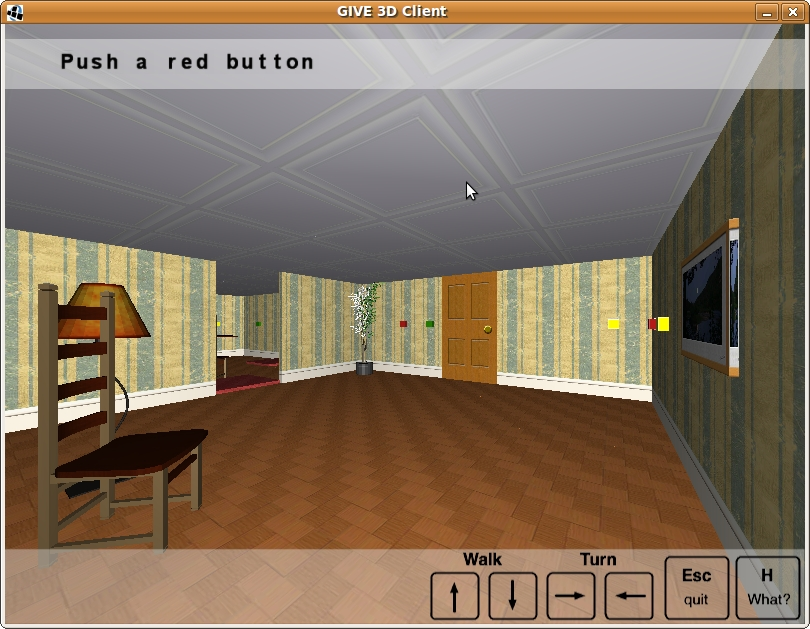
\includegraphics[width=1\linewidth]{give-3D.jpg} 
\end{center}
\caption{The user's view of the 3D world\label{3d-world}}
\end{figure}

On the top of the picture, the current instruction given by the
instruction giving system is displayed. The picture shows a closed
door and an open door that has an activated alarm (that looks like a
red tile) in the doorway. There are five visible buttons in this room
(two yellow, two red and one green) and the instruction giver is
instructing the user to press a red button. Pressing a button can have
different effects such as opening a door, deactivating an alarm, etc.

The characteristics of the world, including the functions of the
buttons, are described in the world specification by the world
designers. The user can move freely around the world (using the direction keys
as indicated in the bottom of the screen) but she can loose the game if she
triggers an alarm. The user can also ask for help pressing `H' if he did not
manage to read or to understand the last instruction.

For the correct definition of the interaction policies of our prototype we need
a corpus that provides examples of typical interactions in the domain. GIVE
provides tools for collecting such corpus in the form of a Wizard of Oz
platform that record all details of the interaction, thus
allowing to easily obtain a corpus of interaction in virtual environments
annotated automatically.

\subsection{The Dialogue System Tasks}

From the collected corpus we will begin the design, implementation and testing
of our dialogue system.  The main components that we will have to design and 
implement can be organized using the traditional four tasks that a dialogue 
system should address: (1) content planning, (2)
generation of referring expressions, (3) management of the interaction context, and
(4) interpretation of user responses. 

\emph{(1) Content Planning:} Given the envisioned setup we described in Section~\ref{intro},
the first task of the system is to obtain a plan to reach the desired goal, from the current state.
The plan will contain physical actions to be performed in the virtual environment. The second
step is to decide how to transmit this sequence of actions to the user. E.g, to decide
how many actions to communicate per instruction, and how to aggregate them
coherently. The result of the action aggregation process can be represented as a
tree describing the task structure at different levels of abstraction. The third
and final step is to decide how to navigate the tree of actions to verbalize the
instructions (for example, post or preorder as
explored in~\cite{foster-etal-ijcai2009}). We will investigate
different aggregation policies (e.g., aggregating actions that
manipulate similar objects) and innovative ways in which to navigate the task tree
(e.g., moving to a lower level of abstraction in case of misunderstandings).
Plan computation can be solved using classical planners~\cite{nau04}.
However, while there are planners that work well when optimized for certain
applications, none provides services such as the generation of alternative
plans, or the generation of incomplete plans in case of the absence of plan.
One of the goals of the project is to design and implement these extensions to 
classical planning algorithms. We will also study the theoretical behavior (e.g., complexity) of
these new algorithms. 

\emph{(2) Generation of Referring Expressions:} Once content planning is
complete, the next step is to generation adequate referring expressions. 
This task involves producing a phrase that describes a referable entity so that the user can
identify it (e.g., ``the vase on the table''). To be
acceptable, these expressions should be ``natural:'' they should be at the same time
sufficiently but not overly constrained, and they should not impose on the user a heavier 
cognitive load than necessary. For example, producing the expression 
``the vase that is not above the chair or sofa or under the
table'' would probably not be acceptable. Areces et al.~\shortcite{AKS08} propose to
use symbolic minimization of the model that represents the state of the world, in
order to obtain logical formulas that describe each object uniquely. In our
project we will implement this method and evaluate it within the dialogue system.

\emph{(3) Management of the Interaction Context:} To manage the use of
the interaction context we will use existing knowledge maintenance systems such as
RACER\footnote{\url{http://www.racer-systems.com}} or Pellet\footnote{\url{http://clarkparsia.com/pellet}}, which support inference tasks such as
definition, maintenance and querying of ontologies. These systems have been used
as inference engines in numerous applications in
the area and, in particular, in dialogue systems for text adventures~\cite{benotti09b}. Once we
have studied the behavior of these inference engines on the task, we will
analyze its limitations and investigate the required extensions.

\emph{(4) Interpretation of User Responses:} The interpretation of user
responses in the unidirectional system is relatively simple: it amounts to
discretizing the continuous flow of user behavior in the 3D world into actions
meaningful for the domain task. In a first
stage, we will use the discretizer provided by GIVE. After evaluating it we can
determine whether or not this module meets the requirements of
our task and what are its limitations. In the bidirectional system, however,
the interpretation of user responses is the task that will require more
attention.
To start with, the bidirectional system should be expanded with capabilities
for  processing statements coming from the user (namely, parsing, semantic
construction, resolution of references, etc.). We will study, in particular, two
types of user contributions: requests for clarification of the instruction
given (what we call `short-term repairs'), and for redefinition of goals (what we
call `long-term repairs'). We will implement short-term repairs
using the approach described in~\cite{purver06}. For long-term repairs we will use the
guidelines of~\cite{blaylock05a}. 

\medskip
A sample interaction with the unidirectional system (that we describe
in~\cite{amoia10}) while guiding the player in
identifying a particular blue button is as follows:
\enumsentence{
System says: Push a blue button. \\
\emph{The user focuses a blue button.} \\ 
System says: Not this one, look for another one. \\
\emph{The user turns and focuses another blue button.} \\
System says: Yes this one! \\
\emph{The user pushes the button.}
}

This interaction illustrates the tasks described above. To begin with, the
verbalization of the instruction ``Push a blue button'' is making explicit one
of the steps of the plan that needs to be performed in order to achieve the
task goal, in this case, taking a trophy from a safe. In order to open the safe
a sequence of buttons need to be pressed. Moreover, the system illustrated
implements a referring strategy which does not uniquely identify the referent
(it's saying ``a blue button'' where there is more than one blue button). We
plan to compare such underspecified strategy with the one proposed in task (2)
in this section. Finally, this example makes evident that the interpretation of
the user responses is crucial even in a linguistically uni-directional system.
The user cannot make linguistic contributions but can change the context by
performing physical acts, the correct interpretation of such acts is essential
if the system is to react coherently to such acts. 
 
\subsection{Evaluation}
To determine the quality of the obtained prototypes we propose to create a
quality model following the ISO/IEC
9126 and 14528 standards for the evaluation of software
products~\cite{ISO9126-1,ISO14598-1}. These standards were successfully applied
to
the Machine Translation domain, resulting in the
\emph{FEMTI\footnote{\url{http://www.issco.unige.ch/femti/}}, Framework for the
Evaluation of
Machine Translation}~\cite{Est2005}. FEMTI
guides evaluators towards creating parameterized evaluation
plans that include various aspects of the to-be-evaluated system and offer a
relevant set of metrics. The identification of relevant metrics can be performed
using various methods, e.g., based on previous
experience~\cite{paradise06,Litman2002}, conducting
surveys or requirement specifications~\cite{Lecoeuche98}, or
collecting such data through Wizard of Oz
experiments~\cite{Dahlback93}.
After developing a quality model, several methodologies to assess
various aspects of the system can be applied: automatic metrics,
subjective metrics or metrics based on the task (to
evaluate both the contribution of each component and the quality of the whole
system). 

The GIVE platform is used every year as a unified framework for evaluating
generation systems. Systems have to generate natural language
instructions and be able to participate in a real-time interaction situated in a
3D environment. The GIVE Challenge is one of the shared tasks endorsed by
ACL's special interests groups in generation, dialogue and semantics. We plan
to participate in the challenge, which will serve as an additional
source of information about aspects of the system that need
improvement.
Once the prototype is evaluated and improved using the results
of this evaluation, we will investigate its use as a virtual language tutor as
described in the next section.

\subsection{An Application: A Virtual Tutor}\label{applications}

The project outcome will be a system capable of giving natural language
instructions situated in a virtual 3D environment. The technology and
theoretical advances of the project could be used in various applications, but
one of the most interesting characteristics we plan to investigate is that, 
a priori, by just changing the linguistic resources, the language of interaction
with the system (input and output) can be changed as desired. After obtaining a
first prototype of an instruction giving dialogue system, 
 we will investigate its use for distance learning,
adapting the system to operate as a foreign language tutor~\cite{Wik09}.

A one-way system that generates instructions in English can be used to test the
user understanding of a foreign language. The correct interpretation of the
instructions can be evaluated from the proper execution of the instructions. The
two-way system will allow the user to formulate clarifications (either in their
native language or in the foreign language). The user may also redefine the
objective to be achieved during the interaction, and thus select the type of
vocabulary he wants to practice.

Virtual worlds (like Second Life) are being rapidly incorporated into
education, both initial and superior~\cite{Doswell05,molk:lear09}. The use of a
virtual tutor has certain advantages over a human tutor.
Engwall~\shortcite{engwall1020} mentioned the following. (1) Amount of
practice: the chance to practice the new language is essential for learning, and
a virtual tutor provides opportunities only limited by the
technological resources. (2) Prestige: a student
may feel embarrassed about making mistakes with a human tutor, and this
might limit his willingness to speak in the foreign language. (3) Augmented
Reality: a virtual
tutor can provide additional material (e.g., examples in context, explanatory
images, etc.) with less effort than a human tutor.


Such a virtual tutor can be used in distance learning. To develop distance learning systems, it is essential to model the user's learning
progress. This requires a system aware of the evolution of the
user, and that takes into account their achievements and their problems. This type
of interaction between user and system can be modeled as a dialogue, which
records the acquired knowledge context (of the user about the course material, and
of the system about to user). The system must be able to interpret requirements, and generate
appropriate responses, for non-experts uses whose knowledge evolves during the
interaction. Moreover, the system must be able to properly represent both the
information concerning the course material, and information about the
evolution of the user. For example, the system must be able to diagnose what
part of the course material should be reviewed from the wrong answers of the
user. Finally, the system must be able to evaluate the user interaction in order
to decide which learning objectives have been achieved. The theoretical and practical
results of the project contribute to solving these difficult
problems.








